\chapter{Asociaciones entre clases}

Se representa mediante una línea continua entre las clases asociadas.\vspace*{0.2cm}
En este caso podemos saber que dado un libro podemos saber sus autores o viceversa.
Las asociaciones entre clases contienen 3 factores (cardinalidad, navegabilidad y multiplicidad).\vspace*{0.2cm}
La \textbf{cardinalidad} es el número de clases asociadas, por defecto, son binarias (cardinalidad = 2).\vspace*{0.2cm}
La \textbf{multiplicidad} indica cuántos objetos de las clases se enlazan, en este caso como mínimo se enlaza 1 y como máximo muchos (1..*). Si no se especifica es 1.\\
La \textbf{navegabilidad} indica el sentido de la relación, por defecto, son bidireccionales pero pueden existir asociaciones de \textit{A → B} o \textit{A ← B} (unidireccionales, donde el extremo de la flecha es el sentido).\vspace*{0.2cm}

Estas asociaciones pueden tener algunas dependencias (agregaciones y composiciones).

\subsection{Implementaciones}
\begin{itemize}
\subsection{Plantilla Implementación 1-N}

\begin{lstlisting}[frame=single]
class A{ //clase con multiplicidad 1
  public:
    //...
    void setB(B&); //enlazamos
    B& getA() const; //objeto B enlazado con A
  private:
    B* b_; //enlace con objeto B
};
class B{ //clase con multiplicidad N
  public:
    //...
    void setA(A&);
    A getB()const;
  private:
    A a_;
};
\end{lstlisting}
\newpage
\subsection{Implementación 1-1}

\begin{figure}[h]
    \centering
	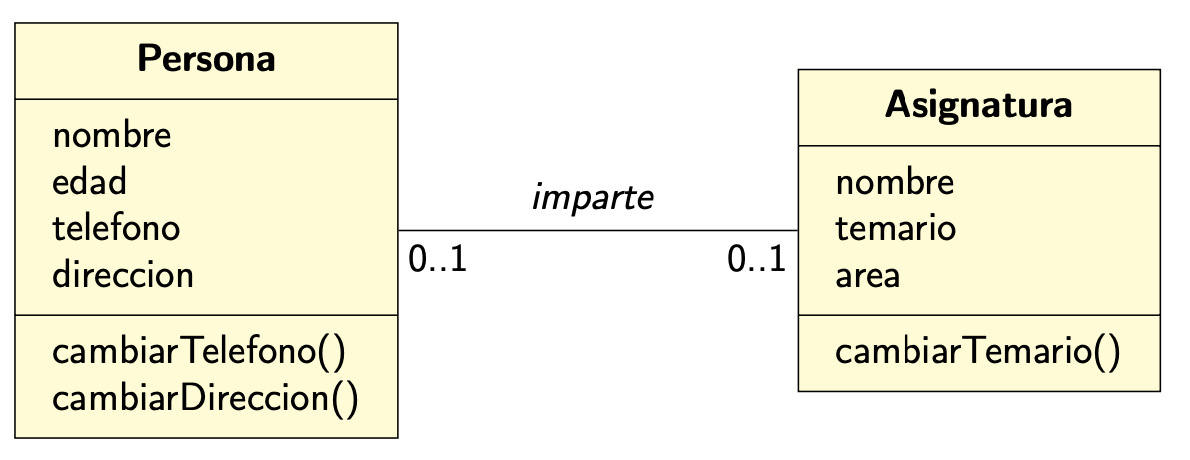
\includegraphics[width=\textwidth]{Imagenes/asociacion1.png}
    \caption{Asociación 1-1}
\end{figure}
\begin{lstlisting}[frame=single]
class Persona{
  public:
    //...
    void setB(Asignatura&); //enlazamos
    
    //objeto Asignatura enlazado con Persona
    Asignatura& getA() const; 
  private:
    Asignatura* b_; //enlace con objeto Asignatura
};
class Asignatura{
  public:
    //...
    void setA(Persona&); //enlazamos
    Persona& getA()const; //objeto Persona enlazado con Asignatura
  private:
    Persona* a_; //enlace con objeto Persona
};

//Implementacion de los metodos
void Persona::setB(Asignatura& b){
    b_ = &b;
}
Asignatura& Persona::getB()const{
    return *b_;
}
//Analogo para obtener Persona
\end{lstlisting}

\newpage
\subsection{Implementación N-M}
\begin{figure}[h]
    \centering
    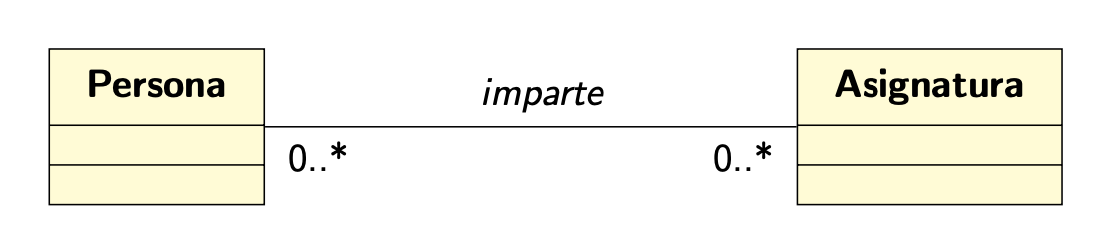
\includegraphics[width=\textwidth]{Imagenes/asociacion2.png}
    \caption{Asociación muchos - muchos}
\end{figure}

\begin{lstlisting}[frame=single]
class Persona{
    public:
        //...
        typedef set<Asignatura*> Bs;
        void setB(Asignatura&);
        const Bs& getA()const;
    private:
        Bs bs_; 
};

class Asignatura{
    public:
        //...
        typedef set<Persona*> As;
        void setA(Persona&);
        const As& getB()const;
    private:
        As as_;
};

void Persona::setB(Asignatura& b){
    as_.insert(&b);
}
const set<Asignatura*>& getA()const{
    return bs_;
}
//Análogo para obtener Persona
\end{lstlisting}


